\chapter{Introduction}

\section{Background}

Cloud-native systems have become the dominant infrastructure for modern software services. Built upon containerization technologies and orchestration platforms such as Kubernetes~\cite{k8s}, these systems fundamentally reshape how applications are developed, deployed, and scaled. According to the Cloud Native Computing Foundation (CNCF), Kubernetes is now adopted by over 84\% of organizations running containerized workloads in production~\cite{cncf2024kubernetes}, with rapid adoption across industries including finance, healthcare, telecommunications, and government~\cite{unyaml2024k8sstats}.

Modern cloud-native deployments are structured as a layered software stack that integrates multiple components across different abstraction levels. At the core, cloud orchestration platforms such as Kubernetes are responsible for scheduling, scaling, and managing the lifecycle of containerized workloads. These platforms rely on container runtimes to operate, specifically high-level Container Runtime Interface (CRI) implementations (e.g., containerd~\cite{containerd}, CRI-O~\cite{crio}) for image management and resource provisioning, which further invoke OCI-compliant low-level runtimes (e.g., runc~\cite{runc}, gVisor~\cite{gvisor}) to enforce process isolation and execute container instances on host systems. Cloud applications are typically deployed within containers or pods, enabling flexible deployment, scalability, and efficient resource utilization.

This architectural decomposition enables the \textit{``build once, run anywhere''} paradigm that underpins cloud-native computing. However, it also introduces a complex and tightly coupled execution environment in which security guarantees depend on the correct interaction of all layers. The resulting system exhibits a broad and heterogeneous attack surface spanning cloud applications, container runtimes, orchestration platforms, and the underlying host operating system. Moreover, the dynamic nature of cloud-native systems further amplifies security risks. Continuous deployment practices, frequent system updates, and the extensive use of third-party dependencies introduce constant changes to system behavior and configuration. These characteristics not only increase the likelihood of vulnerabilities but also complicate security analysis and defense, as assumptions about system behavior may quickly become outdated in practice.

\section{Threat Landscape in Cloud}

The multi-layered architecture of cloud-native systems gives rise to a complex and interconnected threat landscape spanning multiple levels of abstraction. As illustrated in \autoref{fig:attacksurface}, cloud systems consist of tightly coupled components across the application layer, container runtime, orchestration platform, and host system. This layered structure not only introduces multiple attack surfaces but also enables threats to propagate across layers, amplifying their impact. For example, an external attacker may initially exploit a vulnerability in a cloud application (e.g., via remote code execution), obtain execution privileges within a container, and subsequently escalate privileges or exploit runtime vulnerabilities to achieve container escape, ultimately compromising the underlying host or even the entire cluster. At the same time, threats are not limited to external adversaries. Insider entities, including malicious or compromised users with legitimate access, can exploit their privileges to conduct internal attacks such as data exfiltration, privilege abuse, or social engineering (e.g., phishing and credential theft). These attacks often operate at higher abstraction levels, leveraging APIs, management interfaces, and organizational workflows, and can be equally damaging due to their broad access scope.

\textbf{Vulnerabilities as the Root Cause.} At the foundation of this threat landscape are vulnerabilities in cloud software components. These vulnerabilities originate from defects in critical infrastructure, including container runtimes, orchestration platforms, and their interactions with the host operating system. Due to the presence of strict privilege boundaries (e.g., between containers and the host), such defects are particularly security-critical. For example, container runtime vulnerabilities such as CVE-2019-5736 and CVE-2024-21626 exploit flaws in low-level execution mechanisms to achieve container escape, allowing attackers to gain host-level privileges. Similarly, orchestration-layer vulnerabilities such as CVE-2018-1002105 enable privilege escalation from low-privileged users to full cluster control. Importantly, these vulnerabilities typically serve as entry points that can be leveraged by attackers to launch multi-stage attacks. As shown in \autoref{fig:attacksurface}, a vulnerability at any layer (e.g., application or runtime) can be exploited to traverse the stack and compromise the entire system.

\textbf{External Attacks.} External attacks are initiated by adversaries without prior access, who exploit exposed interfaces to penetrate the system. In cloud-native environments, attackers typically begin at the application or API level (e.g., web services, Kubernetes API server), as illustrated on the left side of \autoref{fig:attacksurface}. A common attack path involves exploiting a vulnerability in a cloud application (e.g., via remote code execution), obtaining execution privileges within a container, and then leveraging additional vulnerabilities or misconfigurations to escalate privileges or perform container escape. Once the attacker reaches the runtime or host level, they may gain control over other containers or even the entire cluster.

This attack process is inherently multi-stage and cross-layer, as initial access is achieved through application-level entry points, while privilege escalation and lateral movement occur through runtime and orchestration components. Real-world campaigns, such as those by TeamTNT, demonstrate how attackers exploit exposed Docker daemons or Kubernetes APIs to deploy malware, steal credentials, and propagate across cloud infrastructures. Existing defenses against such attacks primarily rely on runtime monitoring and detection, particularly log-based anomaly detection techniques that aim to identify deviations from normal system behavior.

\textbf{Insider Threats.} In contrast to external attacks, insider threats originate from entities that already possess legitimate access to the system. As shown on the right side of \autoref{fig:attacksurface}, insiders interact with cloud systems through high-level control interfaces, such as administrative commands (e.g., \texttt{kubectl}), user operations, and API-driven workflows. This allows them to directly access and manipulate system components without needing to exploit external vulnerabilities. Insider threats can manifest as malicious actions (e.g., data exfiltration, privilege abuse, sabotage) or unintentional behaviors (e.g., misconfigurations, credential leakage). Unlike external attacks, which typically follow a bottom-up escalation path, insider threats operate in a top-down manner: privileged users can directly issue commands to the orchestration layer, affecting containers, workloads, and system configurations at scale. For example, an insider with administrative privileges can modify deployment configurations, access sensitive data, or introduce backdoored workloads without triggering traditional perimeter defenses.

Detecting insider threats is particularly challenging because their activities often resemble legitimate operations. Moreover, as these actions are executed through standard interfaces (e.g., API calls or CLI commands), distinguishing malicious intent from benign behavior requires fine-grained behavioral modeling. Existing approaches primarily rely on insider threat detection (ITD) techniques based on user activity analysis, but their effectiveness is limited by the lack of realistic data capturing complex human behaviors.

\begin{figure}[t]
    \centering
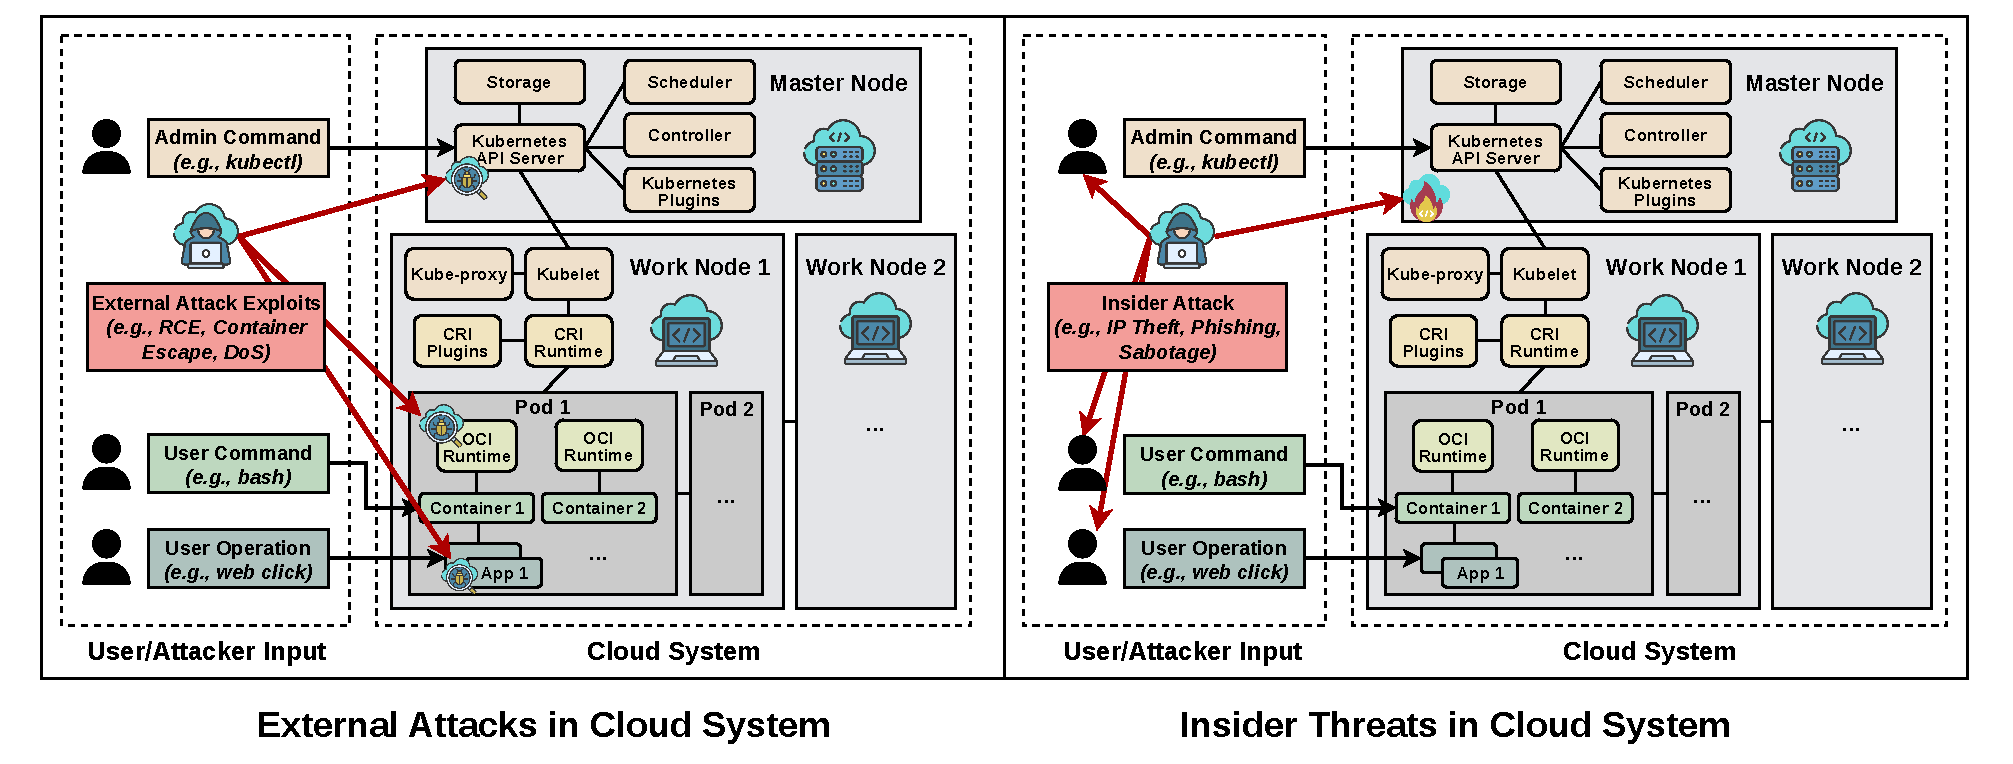
\includegraphics[width=1\linewidth]{Figures/Threats.pdf}
    \caption{Different threats in cloud systems.}
    \label{fig:attacksurface}
\end{figure}

\section{Limitations of Existing Approaches}

Despite extensive efforts to defend against the aforementioned threats, existing approaches primarily follow two directions: (1) securing cloud infrastructure through vulnerability detection and testing, and (2) detecting attacks via system-level monitoring and anomaly detection. However, these approaches exhibit fundamental limitations when applied to cloud-native environments:

\begin{itemize}
    \item \textbf{Lack of Systematic Understanding of Cloud Runtimes.} Existing studies mainly focus on identifying individual vulnerabilities, without a comprehensive understanding of defect patterns in critical cloud components such as container runtimes. Consequently, the characteristics and security implications of these defects remain underexplored, and the effectiveness of existing testing techniques is not well understood.

    \item \textbf{Limited Robustness of Attack Detection.} Most attack detection methods are developed under stationary assumptions, whereas cloud-native systems continuously evolve due to application updates, infrastructure changes, and configuration variations. Such dynamics introduce persistent distribution shifts, which can significantly degrade detection performance in practice.

    \item \textbf{Lack of Data for Insider Threat Analysis.} Insider threat detection is fundamentally constrained by the lack of realistic and high-fidelity data. Privacy and confidentiality restrictions limit access to real-world datasets, while existing public datasets fail to capture complex human-driven behaviors, hindering effective modeling and evaluation.
\end{itemize}

These limitations reveal a fundamental gap between existing security approaches and the dynamic, heterogeneous nature of cloud-native systems, motivating the need for more systematic and integrated solutions.

\section{Research Problems}

To bridge the above gaps, this dissertation advances the security of cloud-native systems along three complementary research directions:

\begin{itemize}
    \item \textbf{Defect Characterization in Cloud Runtimes.} This work investigates how to systematically characterize defect patterns in container runtime systems, analyze their root causes and security implications, and evaluate the effectiveness of existing testing techniques.

    \item \textbf{Robust Detection of External Attacks under Dynamic Environments.} This work studies how cloud-specific distribution shifts, induced by application evolution and infrastructure changes, affect detection performance, and explores shift-aware adaptation techniques (e.g., continual learning) to improve robustness.

    \item \textbf{Data-Driven Insider Threat Detection.} This work investigates how to systematically reenact insider threat scenarios and generate high-fidelity, behaviorally diverse data to enable more effective and generalizable detection.
\end{itemize}

\section{Overview of this Dissertation}

To address these research problems, this dissertation adopts a threat-driven and vertically integrated approach to cloud-native security, as illustrated in~\autoref{fig:thesis-overview}.

\begin{figure}[t]
\centering
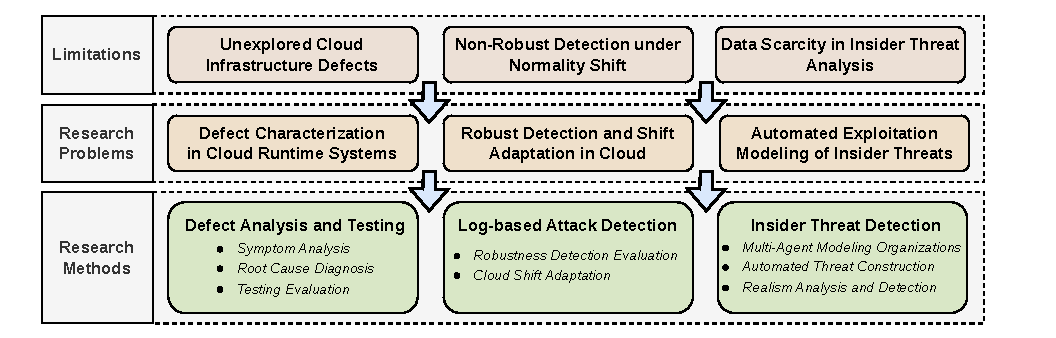
\includegraphics[width=1.0\textwidth]{Figures/Thesis-Overview.pdf}
\caption{{Overview of this dissertation.}}
\label{fig:thesis-overview}
\end{figure}

For real-world cloud-native systems, this dissertation investigates security challenges through a progressive perspective, moving from underlying software defects to externally observable attacks and, ultimately, to insider threats. First, it examines defects in critical cloud infrastructure components, particularly container runtime systems, with the goal of systematically characterizing defect patterns and understanding the limitations of existing testing techniques in detecting them. 

Second, building upon this foundation, it investigates the effectiveness of existing attack detection methods under dynamic system conditions when vulnerabilities are exploited by adversaries at runtime. In particular, it analyzes how evolving system behaviors, such as application updates and infrastructure changes, affect detection performance, and explores continual learning techniques to improve robustness in non-stationary environments. 

Finally, it addresses insider threat analysis within organizational boundaries. To overcome the lack of realistic data, it develops an LLM-based multi-agent framework that simulates organizational activities, generating both adversarial insider behaviors and behaviorally diverse, high-fidelity benign activities. This enables more generalizable insider threat analysis.

Through this progression, the dissertation integrates defect understanding, robust attack detection, and insider threat analysis into a unified and vertically structured framework for securing cloud-native systems.

\section{Main Contributions}

This dissertation makes the following key contributions:

\section{Publications}
The core of this dissertation is built upon the following first-authored research works:

\section{Dissertation Structure}

The remainder of this dissertation is organized as follows.